\section{Import/Export From Other Formats}
\label{sec:pgfplots:importexport}
This section contains information of how to single pictures into separate \pdf\ graphics files (or \eps\ graphics files). Furthermore, it explains a matlab (tm) script which allows to convert from matlab to \PGFPlots.

\subsection[Export to pdf/eps]{Export to {\normalfont\pdf/\eps}}
\label{sec:pgfplots:export}
It is possible to export images to single \pdf-documents using routines of \pgfname\ and/or \Tikz.

\subsubsection{Using the Automatic Externalization Framework of \Tikz}
\begin{pgfplotslibrary}{external}
\pgfkeys{
	/pdflinks/search key prefixes in/.add={/tikz/external/,}{}
}
	The |external| library offers a convenient method to export every single |tikzpicture| into a separate~|.pdf| (or~|.eps|). Later runs of \LaTeX\ will simply include these graphics, thereby reducing typesetting time considerably.

	\paragraph{Technical foreword:}
	The |external| library has been written by Christian Feuers\"anger (author of \PGFPlots). It has been contributed to \Tikz\ as general purpose library, so the reference documentation along with all tweaks can be found in~\cite[Section ``Externalization Library'']{tikz}. The command |\usepgfplotslibrary{external}| is actually just a wrapper which loads |\usetikzlibrary{external}| or, if this library does not yet exist because the installed \pgfname\ has at most version $2.00$, it will load a copy which is shipped with \PGFPlots.

	The |external| library has been designed such that \emph{no changes} to the document as such are necessary. The idea is as follows:
\begin{enumerate}
	\item Every |\begin{tikzpicture}| $\dotsc$ |\end{tikzpicture}| gets a file name. The file name can be assigned manually with |\tikzsetnextfilename|\marg{output file name} or automatically, in which case \meta{tex file name}|-figure|\meta{number} is used with an increasing \meta{number}.
	
	\item The library writes the resulting images using system calls of the form |pdflatex --jobname |\marg{output file name} automatically, using the write18 system call of \TeX. It is the same framework which can be used to call |gnuplot|.
\end{enumerate}
The only steps which are necessary is to use

\pgfmanualpdflabel{\textbackslash tikzexternalize}{}%
|\usepgfplotslibrary{external}|

|\tikzexternalize|\marg{the main file name}

\noindent where \meta{the main file name} is the name of your |.tex| file (without the extension |.tex|). No further modification to the document is necessary. Suppose we have a file called |test.tex|:
\begin{codeexample}[code only]
\documentclass{article}

\usepackage{pgfplots}

\usepgfplotslibrary{external}
\tikzexternalize{test}

\begin{document}
	\begin{figure}
		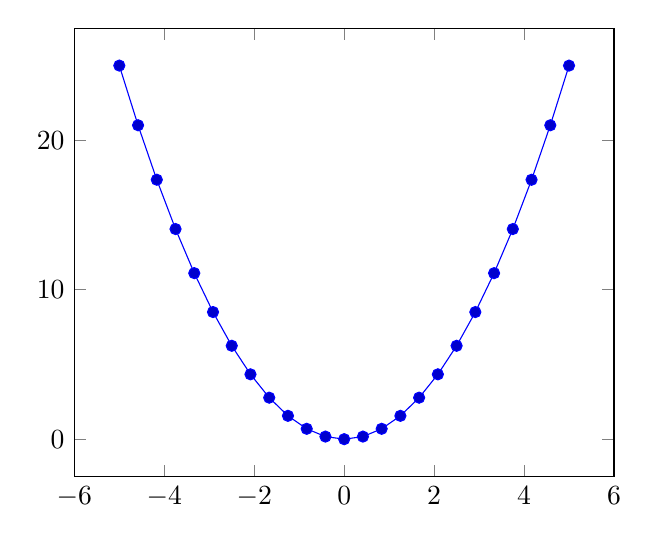
\begin{tikzpicture}
		\begin{axis}
			\addplot {x^2};
		\end{axis}
		\end{tikzpicture}
	\caption{Our first external graphics example}
	\end{figure}

	\begin{figure}
		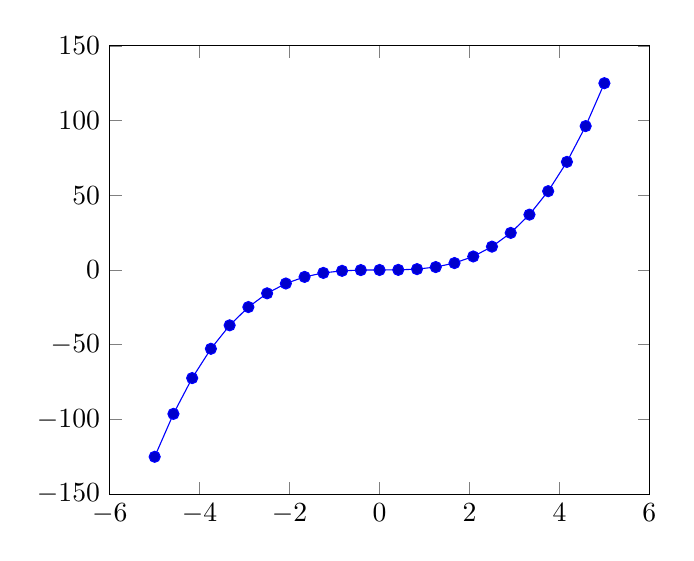
\begin{tikzpicture}
		\begin{axis}
			\addplot {x^3};
		\end{axis}
		\end{tikzpicture}
	\caption{A second graphics}
	\end{figure}
\end{document}
\end{codeexample}
\noindent To enable the system calls, we type
\begin{codeexample}[code only]
pdflatex -shell-escape test
\end{codeexample}
\noindent and \LaTeX\ will now generate the required graphics files |test-figure0.pdf| and |test-figure1.pdf| automatically. Any further call to |pdflatex| will simply use |\includegraphics| and the |tikzpicture|s as such are no longer considered.

If a figure shall be remade, one can simply delete all or selected graphics files and re-generate them. Alternatively, one can use the command |\tikzset{external/force remake}| somewhere in the document to remake every following picture automatically.

There are three ways to modify the file names of externalized figures:
\begin{itemize}
	\item Changing the overall file name using a |prefix|,
	\item Changing the file name for a single figure using |\tikzsetnextfilename|,
	\item Changing the file name for a restricted set of figures using |figure name|.
\end{itemize}
\begin{key}{/tikz/external/prefix=\marg{file name prefix} (initially empty)}
	A shortcut for |\tikzsetexternalprefix|\marg{file name prefix}, see below.
\end{key}

\begin{command}{\tikzsetexternalprefix\marg{file name prefix}}
	Assigns a common prefix used by all file names. For example,
\begin{codeexample}[code only]
\tikzsetexternalprefix{figures/}
\end{codeexample}
	will prepend |figures/| to every external graphics file name.
\end{command}

\begin{command}{\tikzsetnextfilename\marg{file name}}
	Sets the file name for the \emph{next} \tikzname\ picture or |\tikz| short command. It will \emph{only} be used for the next picture.

	Pictures for which no explicit file name has been set will get automatically generated file names.

	Please note that |prefix| will still be prepended to \marg{file name}.
\begin{codeexample}[code only]
\documentclass{article}
% main document, called main.tex
\usepackage{tikz}

\usepgfplotslibrary{external}
\tikzexternalize[prefix=figures/]{main} % provide the file's real name

\begin{document}

\tikzsetnextfilename{firstplot}
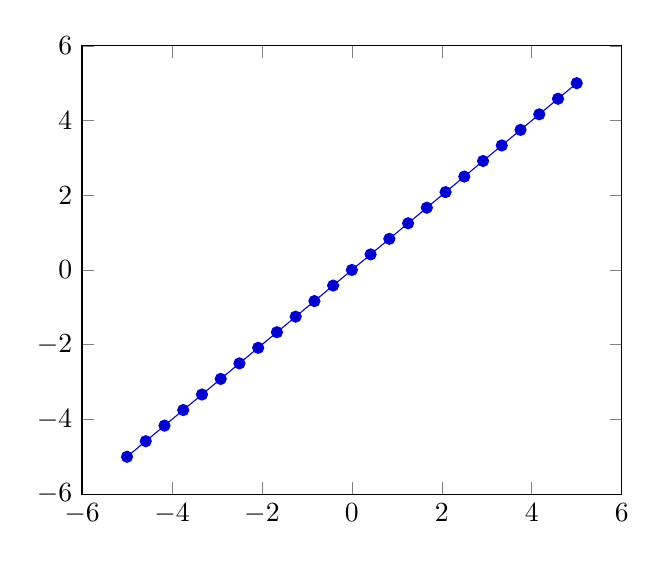
\begin{tikzpicture} % will be written to 'figures/firstplot.pdf'
\begin{axis}
	\addplot {x};  	
\end{axis}
\end{tikzpicture}


\begin{tikzpicture} % will be written to 'figures/main-figure0.pdf'
   \draw[help lines] (0,0) grid (5,5);
\end{tikzpicture}
\end{document}
\end{codeexample}
\begin{codeexample}[code only]
pdflatex -shell-escape main
\end{codeexample}
\end{command}

\begin{key}{/tikz/external/figure name=\marg{name}}
	Changes the names of \emph{all} following figures. It is possible to change |figure name| during the document using |\tikzset{external/figure name|=\marg{name}|}|. A unique counter will be used for each different \marg{name}, and each counter will start at $0$.

	The value of |prefix| will be applied after |figure name| has been evaluated.
\begin{codeexample}[code only]
\documentclass{article}
% main document, called main.tex
\usepackage{tikz}

\usepgfplotslibrary{external}
\tikzexternalize{main} % provide the file's real name

\begin{document}

% will be written to 'main-figure0.pdf'
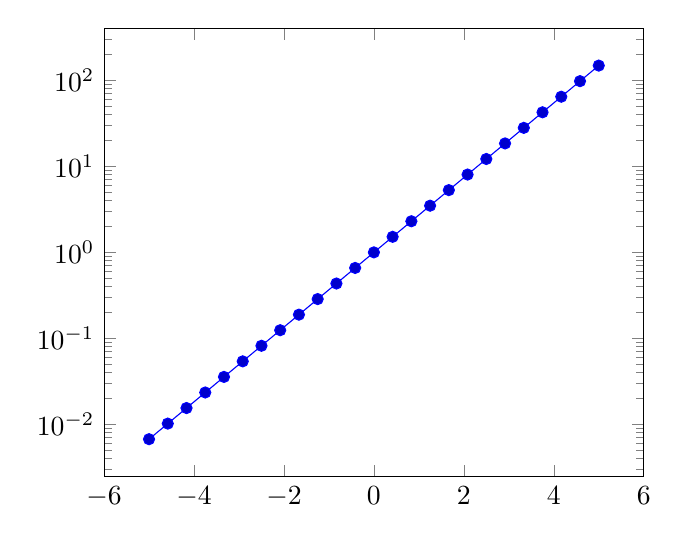
\begin{tikzpicture} 
\begin{semilogyaxis}
	\addplot {exp(x)};
\end{semilogyaxis}
\end{tikzpicture}

{
  \tikzset{external/figure name={subset_}}
  A simple image is \tikz \fill (0,0) circle(5pt);. % will be written to 'subset_0.pdf'

  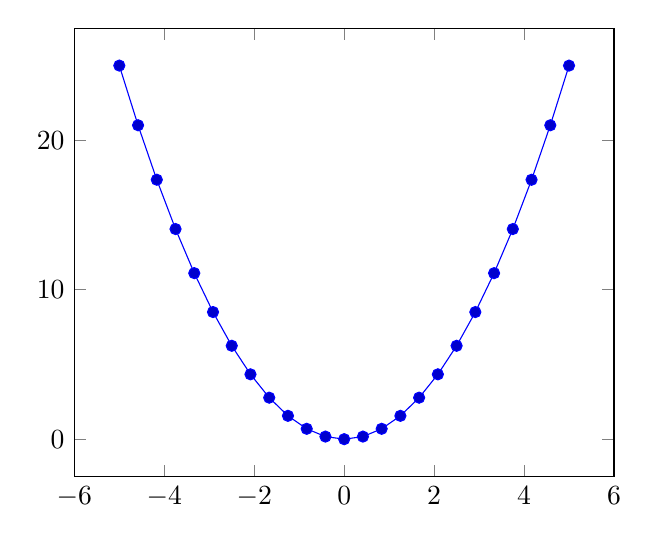
\begin{tikzpicture} % will be written to 'subset_1.pdf'
     \begin{axis}
	 	\addplot {x^2};
	\end{axis}
  \end{tikzpicture}
}% here, the old file name will be restored:

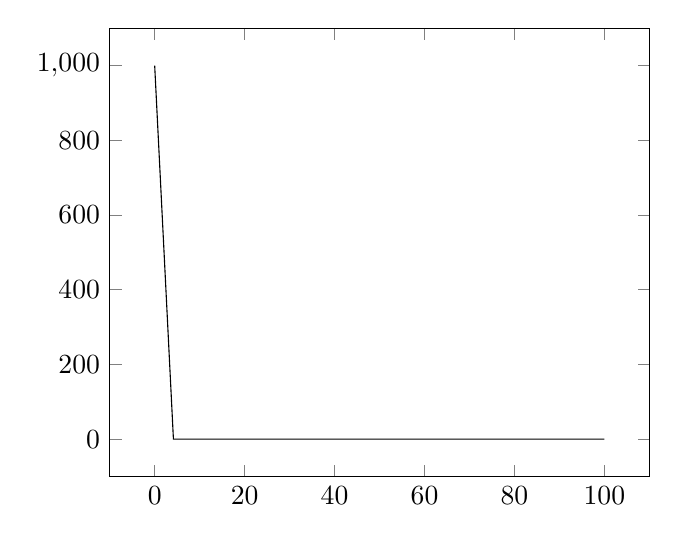
\begin{tikzpicture} % will be written to 'main-figure1.pdf'
   \begin{axis}
   		\addplot[domain=1e-3:100] {1/x};
	\end{axis}
\end{tikzpicture}
\end{document}
\end{codeexample}
	The scope of |figure name| ends with the next closing brace (as all values set by |\tikzset| do).

	Remark: Use |\tikzset{external/figure name/.add={prefix_}{_suffix_}}| to add a |prefix_| and a |_suffix_| to the actual value of |figure name|.
\end{key}


\begin{key}{/tikz/external/system call=\marg{template}}
\label{extlib:systemcall:option}
	A template string used to generate system calls. Inside of \marg{template}, the macro |\image| can be used as placeholder for the image which is about to be generated while |\texsource| contains the main file name.

	The default is 
\begin{codeexample}[code only]
\tikzset{external/system call={pdflatex -shell-escape -halt-on-error 
    -interaction=batchmode -jobname "\image" "\texsource"}
\end{codeexample}

	For |eps| output, you can (and need to) use
\begin{codeexample}[code only]
\tikzset{external/system call={latex -shell-escape -halt-on-error
    -interaction=batchmode -jobname "\image" "\texsource"; 
    dvips -o "\image".ps "\image".dvi}}
\end{codeexample}
	
	The argument \marg{template} will be expanded using |\edef|, so any control sequences will be expanded. During this evaluation, `|\\|' will result in a normal backslash, `|\|'. Furthermore, double quotes `|"|', single quotes `|'|', semicolons and dashes `|-|' will be made to normal characters if any package uses them as macros. This ensures compatibility with the |german| package, for example.
\end{key}

The complete reference documentation and remaining options are documented in~\cite[``Externalization Library'']{tikz}. This reference also contains information about
\begin{itemize}
	\item how to remake selected figures with \declareandlabel{force remake} and \declareandlabel{remake next},
	\item how to disable the externalization partially with \declareandlabel{export}|=false| or completely with |\tikzexternaldisable|,
	\item how to optimize the speed of the conversion process using |\tikzset{optimize command away=\myExpensiveMacro}|,
	\item how to typeset such a document without \pgfname\ installed or
	\item how to provide work-arounds with |.pdf| images and bounding box restrictions.
\index{External Graphics!Bounding Box Issues}
\index{Bounding Box Control!Image Externalization Problems}
\end{itemize}
\end{pgfplotslibrary}

\subsubsection[Using the Externalization Framework of PGF By Hand]{Using the Externalization Framework of {\normalfont\pgfname} ``By Hand''}
Another way to export \TeX-pictures to single graphics files is to use the externalization framework of \pgfname, which requires more work but works more generally than the |external| library.
The basic idea is to encapsulate the desired parts with

\declareandlabel{\beginpgfgraphicnamed}\marg{output file name}

\meta{picture contents}

\declareandlabel{\endpgfgraphicnamed}. 

\noindent Furthermore, one needs to tell \pgfname\ the name of the main document using

\declareandlabel{\pgfrealjobname}\marg{the real job's name}

\noindent in the preamble. This enables two different modes: 
\begin{enumerate}
	\item The first is the normal typesetting mode. \LaTeX\ checks whether a file named \marg{output file name} with one of the accepted file extensions exists -- if that is the case, the graphics file is included with |\pgfimage| and the \meta{picture contents} is skipped. If no such file exists, the \meta{picture contents} is typeset normally. This mode is applied if |\jobname| equals \marg{the real job's name}.
	\item The second mode applies if |\jobname| equals \marg{output file name}, it initiates the ``conversion mode'' which is used to write the graphics file \marg{output file name}. In this case, \emph{only} \meta{picture contents} is written to |\jobname|, the complete rest of the \LaTeX\ is processed as normal, but it is silently discarded.

	This mode needs to be started manually with |pdflatex --jobname |\meta{output file name} for every externalized graphics file.
\end{enumerate}
A complete example may look as follows.
\begin{codeexample}[code only]
\documentclass{article}

\usepackage{pgfplots}

\pgfrealjobname{test}

\begin{document}
	\begin{figure}
		\beginpgfgraphicnamed{testfigure}
		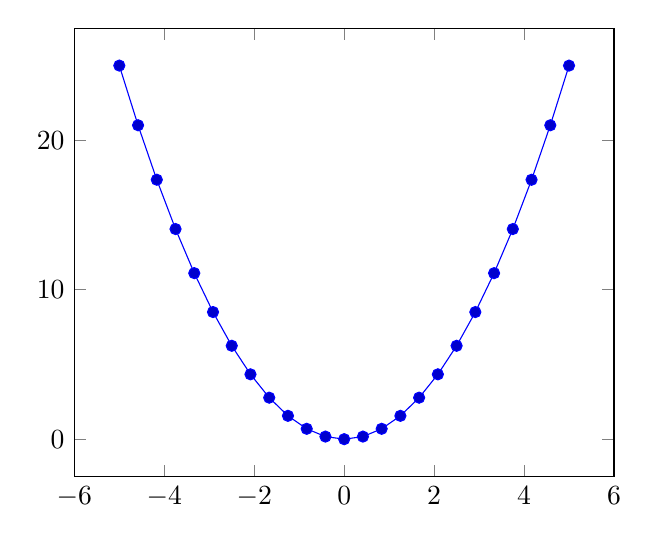
\begin{tikzpicture}
		\begin{axis}
			\addplot {x^2};
		\end{axis}
		\end{tikzpicture}
		\endpgfgraphicnamed
	\caption{Our first external graphics example}
	\end{figure}

	\begin{figure}
		\beginpgfgraphicnamed{testfigure2}
		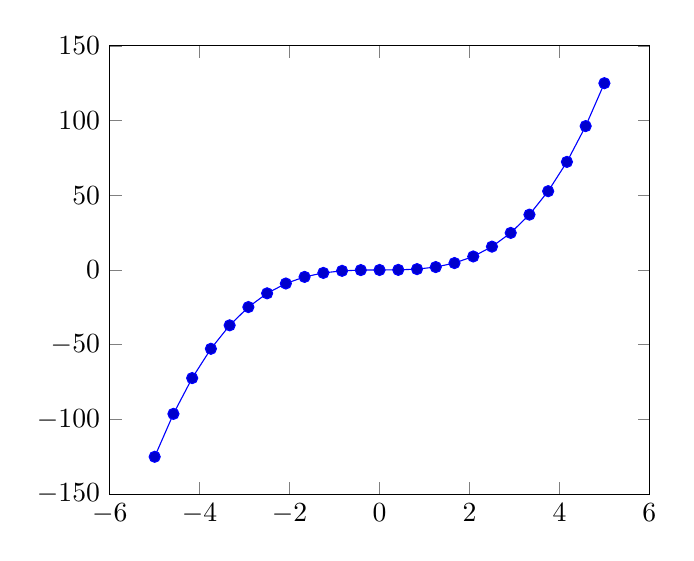
\begin{tikzpicture}
		\begin{axis}
			\addplot {x^3};
		\end{axis}
		\end{tikzpicture}
		\endpgfgraphicnamed
	\caption{A second graphics}
	\end{figure}
\end{document}
\end{codeexample}
\noindent The file is named |test.tex|, and it is processed (for example) with
\begin{codeexample}[code only]
pdflatex test	
\end{codeexample}
\noindent Now, we type
\begin{codeexample}[code only]
pdflatex --jobname testfigure test	
pdflatex --jobname testfigure2 test	
\end{codeexample}
\noindent to enter conversion mode. These last calls will \emph{only} write the contents of our named graphics environments, one for \marg{testfigure} and one for \marg{testfigure2} into the respective output files |testfigure.pdf| and |testfigure2.pdf|.

In summary, one needs |\pgfrealjobname| and calls |pdflatex --jobname |\marg{graphics file} for every externalized graphics environment. Please note that it is absolutely necessary to use the syntax above, \emph{not} |\begin{pgfgraphicnamed}|.

These steps are explained in much more detail in Section``Externalizing Graphics'' of~\cite{tikz}.  This reference also contains information about how to typeset such a document without \pgfname\ installed.

I once attempted to write a unix \texttt{bash}--script |pgf2pdf.sh| which simplifies these steps in case that every externalized graphics environment is placed into a separate file |.pgf|. Interested readers find it in the installation tree.

\paragraph{Attention:} Do not forget a correct |\pgfrealjobname| statement! If it is missing, externalization simply won't work. If it is wrong, any call to \LaTeX\ will produce empty output files.


\subsection{Exporting Mesh Data From Matlab To \PGFPlots}
While it is easy to write Matlab vectors to files (using |save P.dat data -ASCII|), it is more involved to export mesh data.

The main problem is to communicate the mesh structure to \PGFPlots.

Here is an example how to realize this task: in Matlab, we have mesh data |X|, |Y| and |Z| which are matrizes of the same size. For example, suppose we have

\begin{codeexample}[code only]
[X,Y] = meshgrid( linspace(-1,1,5), linspace(4,5,10) );
Z = X + Y;
surf(X,Y,Z)
\end{codeexample}
\noindent as data. Then, we can generate an $N \times 3$ table containing all single elements in column--wise ordering with

\begin{codeexample}[code only]
data = [ X(:) Y(:) Z(:) ]
save P.dat data -ASCII
\end{codeexample}
\noindent where the second command stores the $N \times 3$ table into |P.dat|. Finally, we can use 

|\addplot3[surf,mesh/rows=10,mesh/ordering=colwise,shader=interp] file {P.dat};|

in \PGFPlots\ to read this data. We need to provide either the number of rows ($10$ here) or the number of columns -- and the ordering (which is |colwise| for Matlab matrizes).

An alternative which is faster in \PGFPlots\ would be to transpose the matrizes in Matlab and tell \PGFPlots\ they are in |rowwise| ordering. So, the last step becomes

\begin{codeexample}[code only]
XX=X'; YY=Y'; ZZ=Z';
data = [ XX(:) YY(:) ZZ(:) ]
save P.dat data -ASCII
\end{codeexample}
\noindent with \PGFPlots\ command

|\addplot3[surf,mesh/cols=10,mesh/ordering=rowwise,shader=interp] file {P.dat};|.

\subsection{matlab2pgfplots.m}
This is a Matlab (tm) script which attempts to convert a matlab figure to \PGFPlots. It requires Matlab version 7.4 (or higher).

The idea is to
\begin{itemize}
	\item use a complete matlab figure as input,
	\item acquire axis labels, axis scaling (log or normal) and legend entries,
	\item acquire all plot coordinates
\end{itemize}
and write an equivalent \texttt{.pgf} file which typesets the plot with \PGFPlots.

The indention is \emph{not} to simulate matlab. It is a first step for a conversion. Type
\begin{lstlisting}
> help matlab2pgfplots
\end{lstlisting}
on your matlab prompt for more information about its features and its limitations.

This script is experimental.

\subsection{matlab2pgfplots.sh}
A \texttt{bash}-script which simply starts matlab and runs 
\begin{lstlisting}
	f=hgload( 'somefigure.fig' );
	matlab2pgfplots( 'outputfile.pgf', 'fig', f );
\end{lstlisting}
See matlab2pgfplots.m above.

\subsection{SVG Output}
It is possible to write every single \Tikz\ picture into a scalable vector graphics (\texttt{.svg}) file. This has nothing to do with \PGFPlots, it is a separate driver of \PGF. Please refer to~\cite[Section ``Producing HTML / SVG Output'']{tikz}.

\subsection{Generate \PGFPlots\ Graphics Within Python}
Mario Orne D\'IAZ ANAD\'ON contributed a small python script |pgfplots.py| which provides a simple interface to generate \PGFPlots\ figures from within python. It can be found in the \PGFPlots\ installation directory, in |pgfplots/scripts/pgfplots/pgfplots.py|; documentation can be found in the file.
